\documentclass{mediumfoils}
%\usepackage{arev} 
\usepackage{ctable}
\usepackage[display]{texpower}
\usepackage{hyperref}
\raggedright

\usepackage{ctable}
\usepackage{fancyvrb}
\usepackage{multirow}

%\usepackage{sfmath}
\newcommand{\mkred}[1]{\textsl{#1}}
\newcommand{\mkgreen}[1]{\textsl{#1}}
\newcommand{\mkblue}[1]{\textsl{#1}}
\newcommand{\mkgrey}[1]{#1}


\graphicspath{{/Users/will/Dropbox/}} 

\talktitle{Computer-Assisted Content Analysis:\\ Assigning Categories to Documents}
\author{\textbf{Will Lowe} (University of Mannheim)}

\date{}
\runningfooter{Texas A\&M Jan 2015}

\begin{document}

\maketitle

%
%How to model categorical $\theta$ without specifying a dictionary and without having a training set?
%
%Example questions: 
%
%Simple case: What proportion of weblogs strongly dislike, dislike, are indifferent to, like or strongly like Kerry as a candidate?
%
%Harder case: How does the balance of topics in a corpus change over time?
%

%\slide{Topic Models 1}

%\centerline{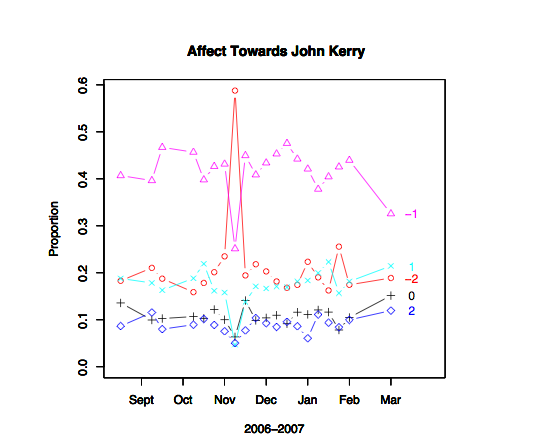
\includegraphics[scale=.8]{pictures/kerry-blogs}}
%

\slide{Menu}

Session 1: Classical Content Analysis

Session 2: 
\ita
\itm Document classification 
\ita
\itm The indirect approach to classification
\itm Evaluation and interpretation
\itm Evaluation for the lazy
\itm The direct approach to classification
\itz
\itz

Session 3: Scaling Models


\slide{Text as Data}

\centerline{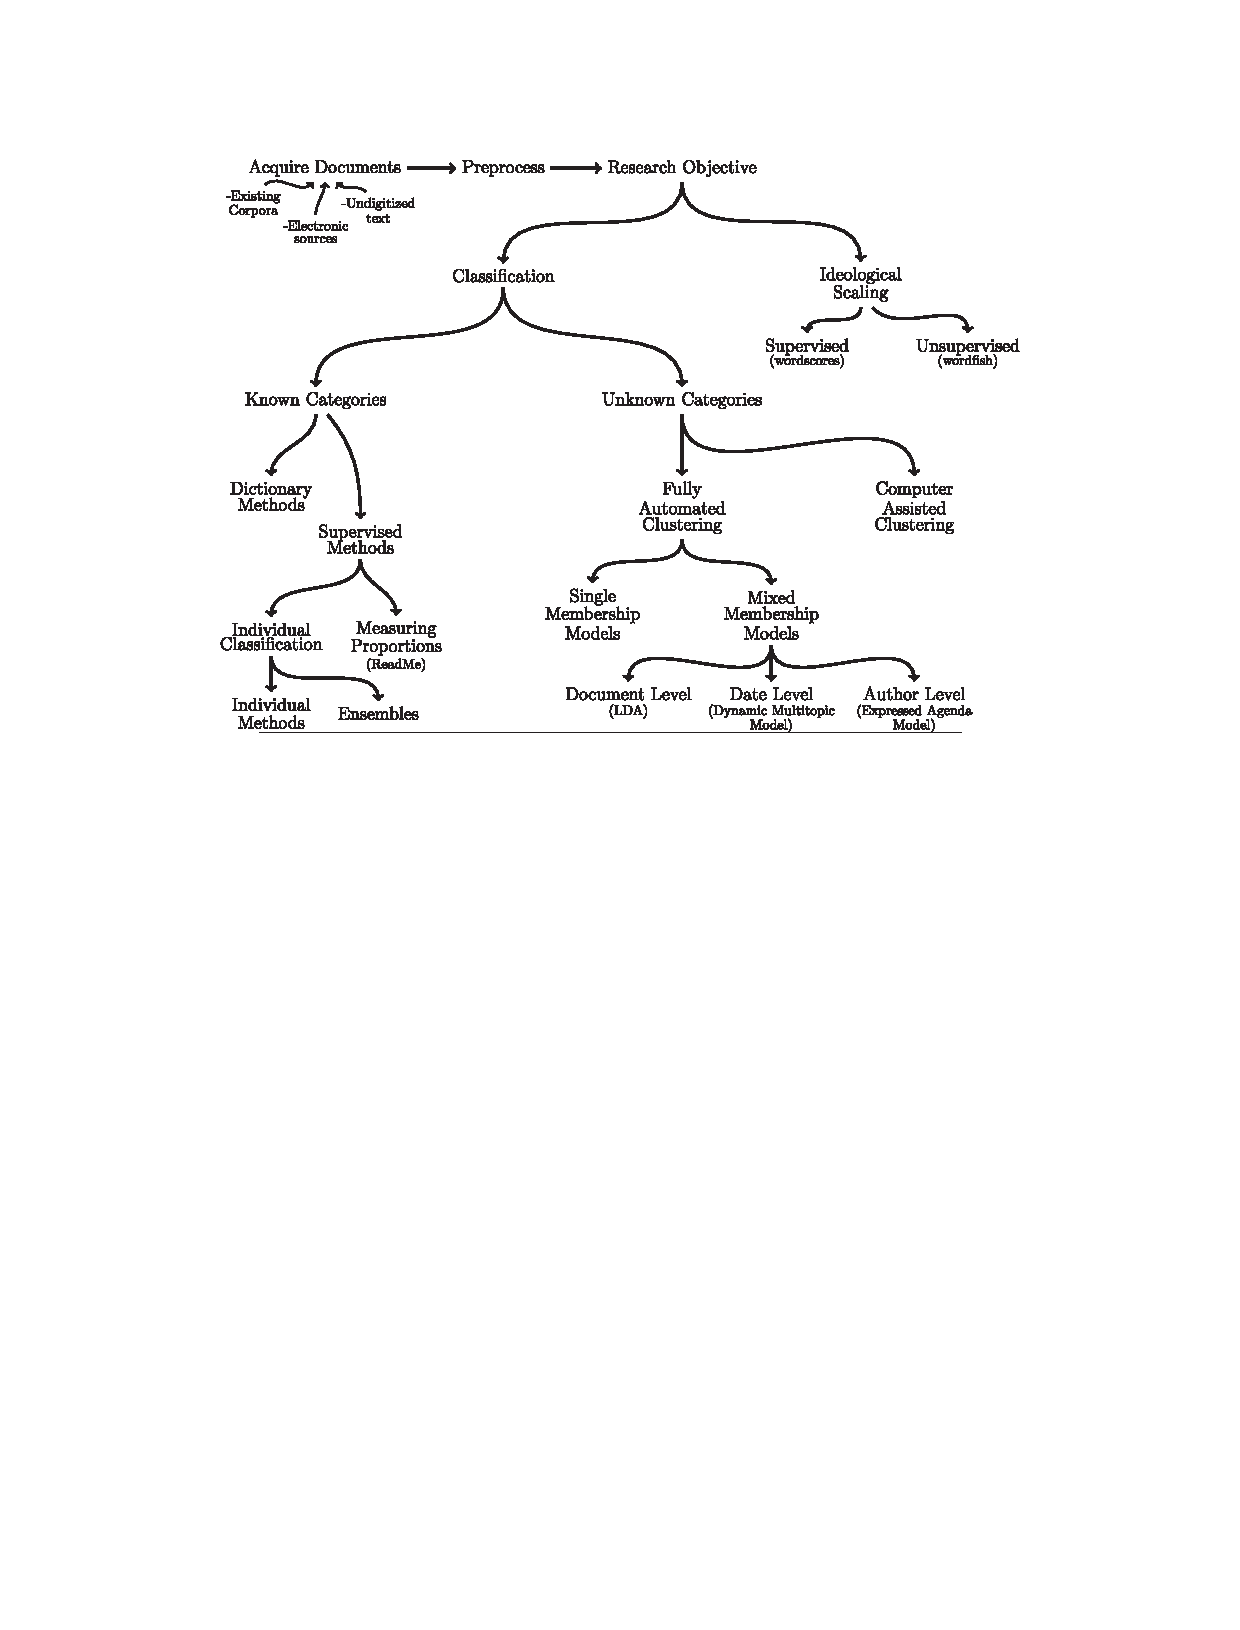
\includegraphics[scale=1.24]{pictures/grimmerovreview.pdf}}
\centerline{\footnotesize Source: Grimmer and Stewart (2013)}




%%%%%%%%%%%%%%%%
%%%%%%%%%%%%%%%%


\slide{Classification Approaches when Categories are Known}

{\bf Examples:}

Are campaign advertisements positive or negative?

What  policy areas do newspaper editorials cover?

Are international statements belligerent or peaceful?

Do court letters represent liberal or conservative positions?

What language is this article written in?

Is this email spam?

\slide{Classification Approaches when Categories are Known}

Yesterday we talked how to do this using a dictionary approach.

An alternative is supervised machine learning methods:
\begin{enumerate}

\item coders categorize a set of documents by hand
\item the algorithm ``learns'' how to sort the documents in categories
\item  characteristics of training set are used  to assign new documents to categories.
\end{enumerate}


\slide{Classification Approaches when Categories are Known}

Assume that each document has a \textit{single} topic Z

Let $\theta_k$ be the \textit{probability} that Z=k for each document

Assume that (some) topic labels are observed



%We can \textit{choose} a style of model\\
%~\\

%\centerline{\includegraphics[scale=.7]{pictures/classification-plate}~~~~~~~~~
%\includegraphics[scale=.7]{pictures/classification-plate2}}

%\centerline{Discriminative Style ~~~~~~~~~~~~~~~~ Generative Style}


\slide{Classification Approaches}

Much of machine learning, computational linguistics, and AI deals with classification problems

Methods: 
\ita
\itm Naive Bayes, Maximum Entropy, Support Vector Machines, Neural Networks, Bagging, Boosting, $\ldots$
\itm We only touch on the issues here\ldots
\itz 

\slide{Classification approaches}

In the simple framework of yesterday 
\ita
\itm $Z$ is the true category of a document 
\itm $\theta$ is be the posterior probability that a document is a particular category
\itz

\slide{Classification approaches}

As before, we have two approaches
\ita
\itm Discriminative: Model $P(Z \mid \{W\}, \beta) = \theta_{z|w}$ directly
\itm Generative: Model $P(\{W\} \mid Z, \beta)$ and $P(Z)=\theta_z$, then get $P(Z \mid \{W\}, \beta) = \theta_{z|w}$ via Bayes theorem
\itz

\slide{Generative vs discriminative training}

\centerline{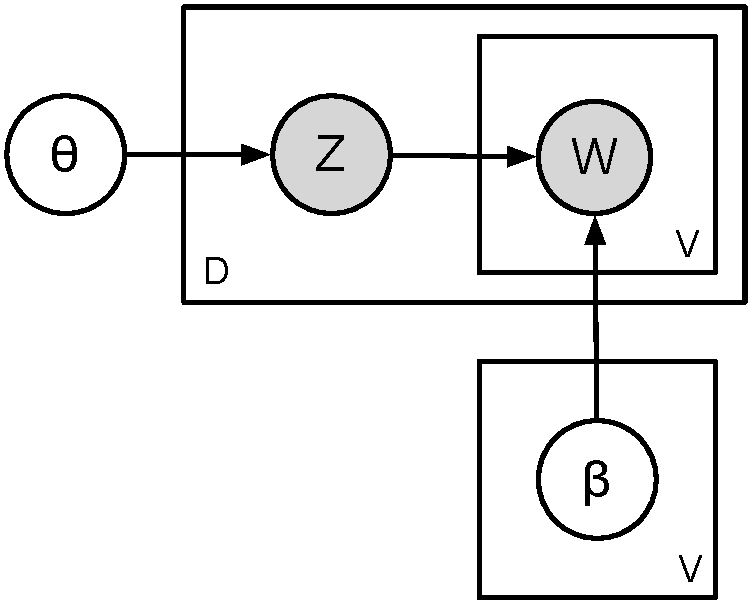
\includegraphics[scale=.7]{pictures/unsupervised-classification} \hfill 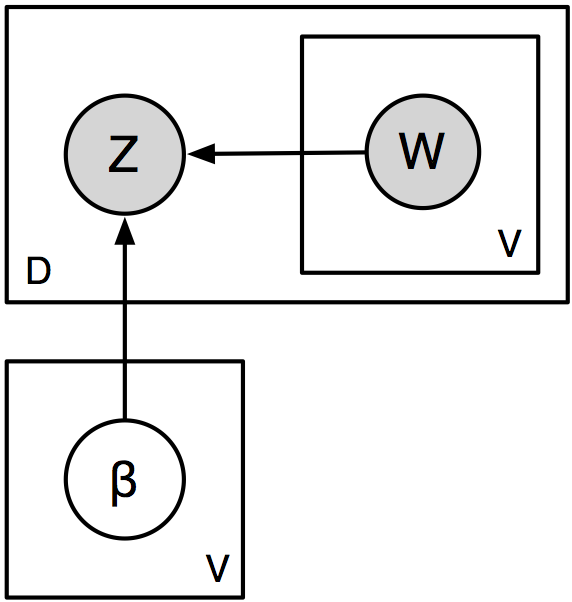
\includegraphics[scale=.7]{pictures/supervised-classification}}

Naive Bayes \hfill Maximum Entropy, etc...

\vfill 

\slide{Generative vs discriminative testing}

\centerline{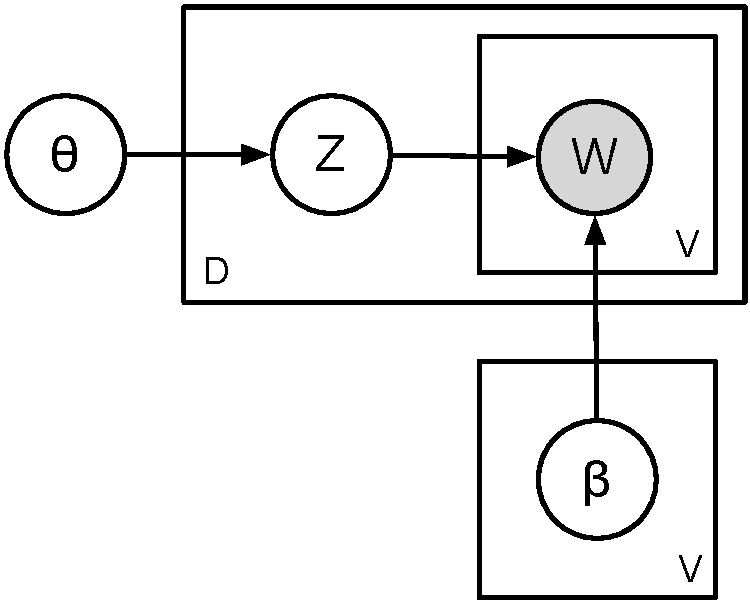
\includegraphics[scale=.7]{pictures/unsupervised-classification-test} \hfill 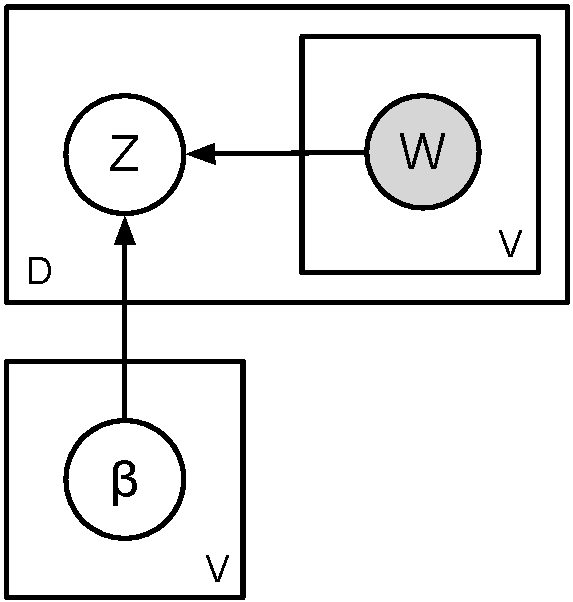
\includegraphics[scale=.7]{pictures/supervised-classification-test}}

Naive Bayes \hfill Maximum Entropy, etc...

\slide{Either way\ldots}

Desirable classification outcome:

\begin{center}
\begin{tabular}{lcc}
      & $P(Z=`\text{Domestic}'\mid \{W\}_d)$ & $P(Z=`\text{Foreign}' \mid \text \{W\}_d)$ \\ \toprule
$D_1$ & 0.75 & 0.25 \\
$D_2$ & 0.82 & 0.18 \\
\ldots & \ldots & \ldots\\
$D_{N-1}$ & 0.02 & 0.98 \\
$D_N$ & 0.45 & 0.55\\ \bottomrule
\end{tabular}
\end{center}

where $\theta_{z|w} = P(Z=z \mid \{W\})$

\slide{The Basic Steps}

\begin{enumerate}

\item Construct a training set
 
(a) create a coding scheme\\
(b) select documents (ideally randomly sampled)

\item Apply the supervised learning method to learn features of a training set and infer labels

\item Validate and classify remaining documents

\end{enumerate}

\slide{Indirect approach: Naive Bayes}

Background:
\ita
\itm Amicus Curiae (friend of the court) briefs are submitted to an appellate court
\itm They usually present a legal argument for or against one of the parties to a case
\itm Amicus Curiae can be submitted by any group that feels that it has a stake in the case
\itz

\slide{Affirmative action}

Evans et al. use cases about the constitutionality of `affirmative action' programs at university level
\ita
\itm Regents of the University of California vs. Bakke (1978)
\itm Grutter vs Bollinger, Lehman, Shields, and the Regents of the University of Michigan (2003)
\itm Gratz and Hamacher vs Bollinger, Lehman, Shields and the Regents of the University of Michigan (2003)
\itz
The arguments are as much \textsl{political} (state vs federal rights, social welfare, constitutional interpretation) as they are \textsl{legal} 

\slide{Affirmative Action}

This work uses document classification to answer two questions
\ita
\itm To what extent can the \textsl{direction} of an AC brief be predicted on the basis of its words?
\itm What can we learn about \textsl{language} of each side of the case? 
\itz

\slide{Naive Bayes}

\textsl{Naive Bayes} is a relatively old ($\sim$1975)  classification method

Suppose you had to guess  whether document $j$ is liberal (Z=`Lib') or conservative (Z=`Con') based on its word profile $\{W\}_j$.

Probability can be derived by applying Bayes theorem:

\begin{align*}
P(Z=\text{`Lib'} \mid \{W\}_j) &~=~ \frac{P(\{W\}_j \mid Z=\text{`Lib'})~P(Z=\text{`Lib'})}{P(\{W\}_j)}
\end{align*}

\slide{Naive Bayes}

\begin{align*}
P(Z=\text{`Lib'} \mid \{W\}_j) &~\propto~ P(\{W\}_j \mid Z=\text{`Lib'})~P(Z=\text{`Lib'})
\end{align*}

We can drop $P(\{W\}_j)$ since it is constant across categories. 

Given a representative training set, estimating $P(Z=L)$ is easy: 

\begin{align*}
\hat{P}(Z=\text{`Lib'})&~=~ \frac{\text{\# training docs that are liberal}}
{\text{\# of training docs}}
\end{align*}

\slide{Naive Bayes}

Estimating the probability that a word profile $\{W\}_j$ occurs given that the document is liberal $P(\{W\}_j\mid Z=\text{`Lib'})$ is more challenging, because any one word profile is likely to occur only once.

Solution: 
\ita
\itm words are assumed to be generated \textit{independently} given the category Z (the `naive' and wrong assumption). 
\begin{align*}
P(\{W\}_j \mid Z=\text{`Lib'}) &~=~ {\prod}_i P(W_i \mid Z=\text{`Lib'})
\end{align*}
\itz
\newpage

\slide{Naive Bayes}

With this assumption, we can estimate the probability of observing a word $i$  given that the document is liberal: proportion of word $i$ in liberal training set.

The classifier then chooses the class Z (Liberal or Conservative) with the highest aggregate probability.

Note that every new word adds a bit of information that re-adjusts the conditional probabilities.

\newpage


\slide{Naive Bayes}



Note that with two classes (here: liberal and conservative)  this has a rather neat interpretation:
\begin{align*}
\frac{P(Z=\text{\text{`Lib'}} \mid \{W\}_j)}
{P(Z=\text{`Con'} \mid \{W\}_j)} = \\
~~~~~~~~~\prod_i \frac{P(W_i \mid Z=\textsl{\text{`Lib'}})}
{P(W_i \mid Z=\textsl{`Con'})}\times \frac{P(Z=\textsl{\text{`Lib'}})}{~P(Z=\textsl{`Con'})}
\end{align*}
Logging this probability ratio, every new word \textsl{adds} a bit of information that pushes the ratio above or below 0

%%%%%%%%%%% check the below works in the real document

%[will@Apparent lib]$ ykcats -dictionary ../../disc.vbpro ../lib/*
%,Dictionary,Dictionary>discrimination,WordCount
%6019_ll01-utf8.txt,26,26,20002
%6020_ll01-utf8.txt,13,13,18722
%[will@Apparent lib]$ ykcats -dictionary ../../disc.vbpro ../con/*
%,Dictionary,Dictionary>discrimination,WordCount
%6019_lc01-utf8.txt,70,70,17368
%6020_lc01-utf8.txt,48,48,17698

% lib = (26+13)/(20002+18722) = 0.001007127
% con = (70+48)/(17368+17698) = 0.003365083
% lib / con = .299

%%%%%%%%%%%

\slide{Naive Bayes}

Example: Naive Bayes with only word class `discriminat*'.
{\small
\begin{align*}
P(W=\text{`discriminat*'} \mid Z=\text{`Lib'}) & = (26+13)/(20002+18722) \approx 0.001\\
P(W=\text{`discriminat*'} \mid Z=\text{`Con'}) & = (70+48)/(17368+17698) \approx 0.003
\end{align*}
}
Assume that liberal and conservative supporting briefs are equally likely (true in the training set)
\begin{align*}
\frac{P(Z=\text{\text{`Lib'}})}{P(Z=\text{`Con'})} & = 1
\end{align*}

Last step:  calculate posterior classification  probabilities for a new document (based on occurrence of this word).

\slide{Naive Bayes}

Amicus brief from `King County Bar Association' containing 3667 words (File 6019\_al18-utf8.txt) and 4 matches to disciminat*.

{\footnotesize
\begin{verbatim}
      that "the state shall not [discriminate] against, or grant preferential treatment
the lingering effects of racial [discrimination] against minority groups in this
 remedy the effects of societal [discrimination]. Another four Justices (Stevens
      that "the state shall not [discriminate] against, or grant preferential treatment
\end{verbatim}
}
\slide{Naive Bayes}

A priori, the probabilities are\ldots

Probability that we observe the word  discriminat* 4 out of 3667 times if the document is liberal: 
{\small
\begin{verbatim}
> dbinom(4, size=3667, prob=0.001007127)
[1] 0.1930602
\end{verbatim}
}

Probability that we observe the word  discriminat* 4 out of 3667 times if the document is conservative:
{\small
\begin{verbatim}
> dbinom(4, size=3667, prob=0.003365083)
[1] 0.004188261
\end{verbatim}
}

Logged probability ratio = 3.83

\newpage

\slide{Naive Bayes}

Conclusion: Seeing 4 instances of discriminat* gives the posterior classification probabilities
\ita
\itm $\theta_\text{liberal}$ = 0.979
\itm $\theta_\text{conservative}$ =  1-0.979=0.021
\itz

This is \textit{quite} confident
\ita
\itm \ldots but other words will be less loaded or push the other way
\itz





\slide{Evaluating Classifiers:\\Accuracy, Precision and Recall}

How can we evaluate how good a supervised classifier works? 

Use the confusion matrix (training set versus machine)


\slide{Evaluating Classifiers:\\Accuracy, Precision and Recall}

\begin{center}
\scalebox{0.7}{
\begin{tabular}{llcc}
\toprule
&&\multicolumn{2}{c}{Machine}\\
\cline{3-4}
&& Liberal & Conservative \\
\midrule
Training Data & Liberal & 40&10\\
& Conservative &40&60\\
\bottomrule
\end{tabular}}
\end{center}

\vspace*{0.5cm}

Accuracy = (40+60)/150 = .66

Precision ($Z_{machine}$=Liberal) = 40/(40+40) = 0.5

Precision ($Z_{machine}$=Cons) = 60/(10+60) = 0.86

Recall ($Z_{training}$=Liberal) = 40/(40+10) = 0.80

Recall ($Z_{training}$=Cons) = 60/(40+60) = 0.60

\newpage

\centerline{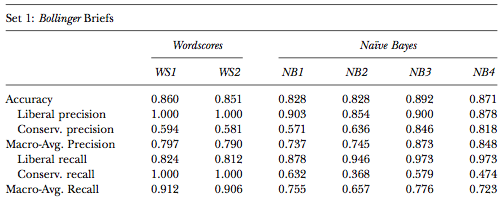
\includegraphics[scale=1.2]{pictures/bolinger}}

\slide{Trading off precision and recall}


\centerline{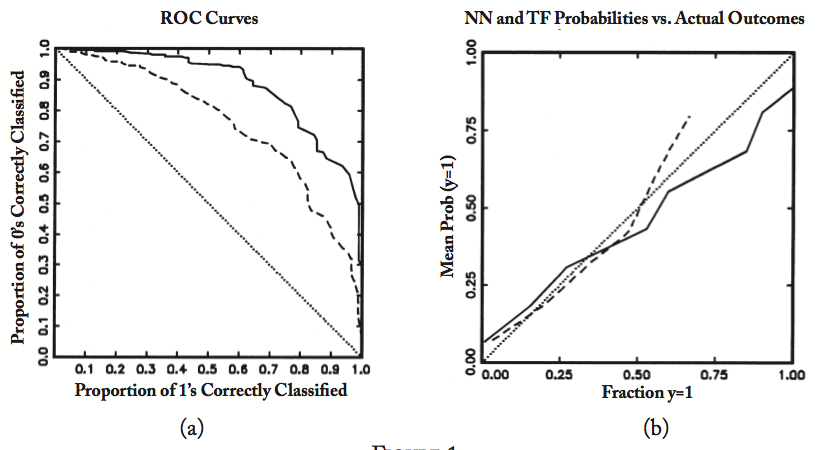
\includegraphics[scale=.7]{pictures/roc-curves}}

(King and Zeng, 2001)

\slide{Evaluation}

All classification models have a secret extra parameter: the \textit{threshold}

\slide{Distinctive Words}

Detecting different rhetorical styles of liberal and conservative groups:

``Liberal groups use language emphasizing the impact of affirmative action polices, while conservative words indicate concern over legal-constitutional limits on administrative procedure'' (Evans et al. 2007, p. 1029)

\newpage

\centerline{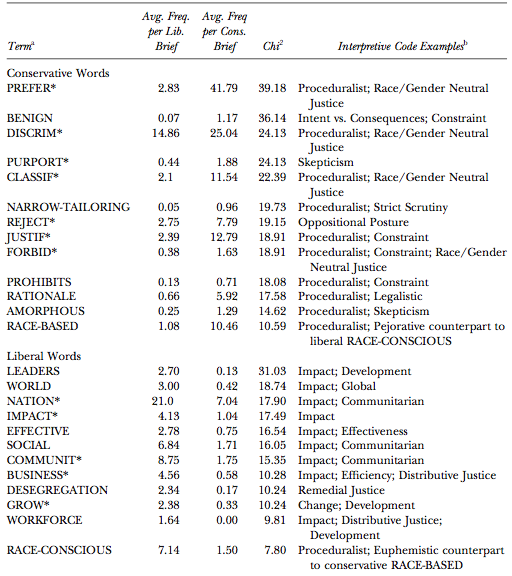
\includegraphics[scale=.9]{pictures/words-evans}}
%
%\slide{Refresher on $\chi^2$}
%
%A $\chi^2$ \textsl{statistic} is computed as 
%\begin{align*}
%\frac{(\text{observed} - \text{expected})^2}{\text{expected}}
%\end{align*}
%In large samples it has a $\chi^2$ \textsl{distribution}.  
%
%For measuring how useful a term would be in a classifier we are more interested in magnitude 
%
%
%\slide{Refresher on $\chi^2$}
%
%\begin{center}
%\begin{tabular}{llll}
%            & purport* & not purport*   & \\ \midrule 
%petitioners & 43       & 166101       & 166144 \\
%respondents & 34       & 673552       & 673586 \\ \midrule
%            & 77       & 839653       & 839730
%\end{tabular}
%\end{center}
%
%If purport* words occurred at the \textsl{same} rate then their expected proportion would be
%\[
%\frac{77}{839730}
%\]
%
%
%If \textit{not} we would estimate the rates as
%\begin{align*}
%\text{conservatives:} && \frac{43}{166144}\\
%\text{liberals:} && \frac{34}{673586}
%\end{align*}
%
%
%The $\chi^2$ asks whether the observed counts are probable under the assumption that words occur at the \textsl{same} rate. Conservatives use purport* words at more than 5 times the rate of liberals.\\
%\begin{align*}
%\frac{43~/~166144}{34~/~673586} & = 5.127
%\end{align*}
%
%\newpage 
%Evans et al. 2007: "Many conservatives doubt that diversity is "narrowly tailored" to achieve a compelling state interest as "purported," or that it actually delivers many of its "alleged" benefits." (p.1030)
%
%
%\newpage
%\centerline{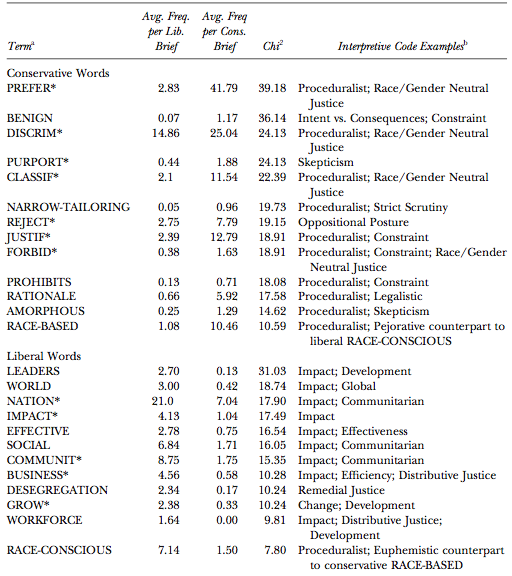
\includegraphics[scale=.9]{pictures/words-evans}}

\slide{Compare and Contrast}

Bara et al. (2007) abortion debate with a thematic dictionary
\begin{center}
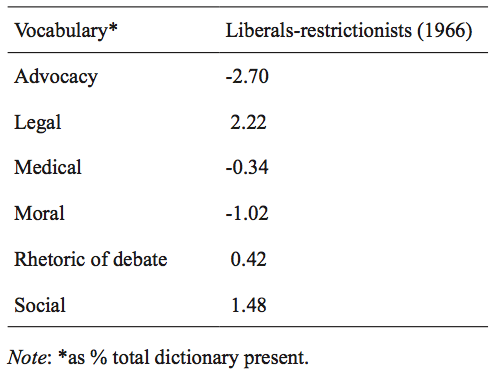
\includegraphics[scale=.6]{pictures/bara-diffs}
\end{center}

\slide{Vocabulary Usage}

We can use known Z to characterize vocabulary usage directly, if we're careful\ldots

Monroe et al. (2008) compare different measures of `partisan vocabulary' in abortion debates
\ita
\itm Simple frequencies will be misleading
\itm They settle for Laplace regularized odds-ratios
\itz

\newpage


\centerline{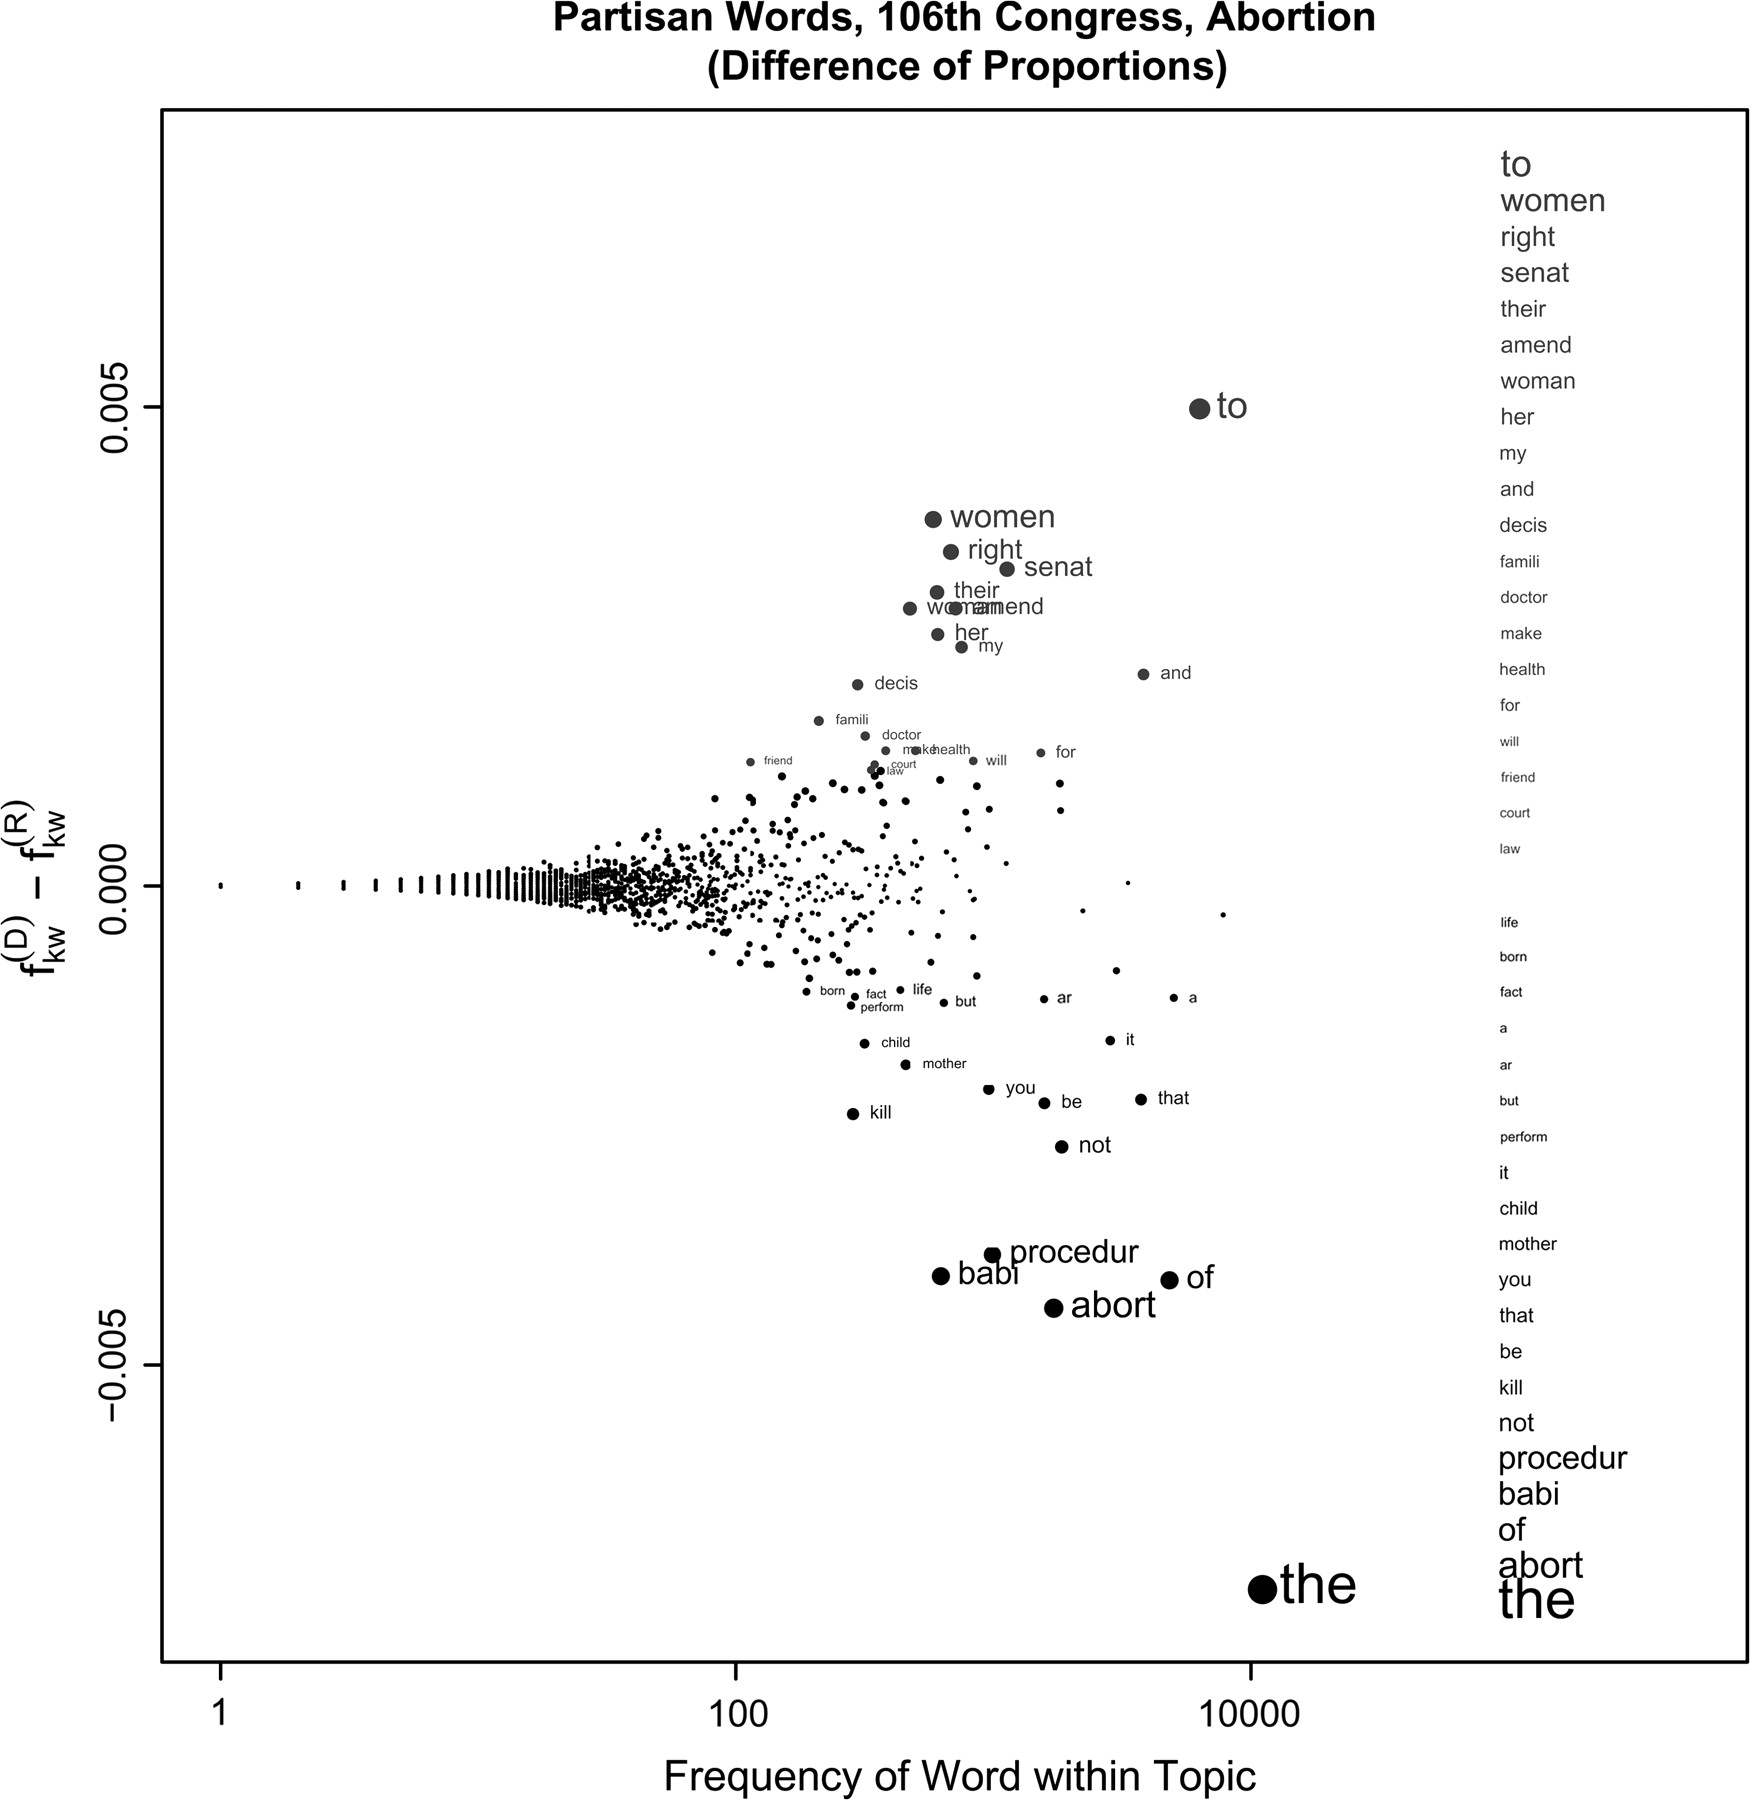
\includegraphics[scale=.2]{pictures/fightin0}}

{\footnotesize Difference of proportions: could result in lack of overall semantic validity due to the overemphasis on high-frequency words, unclear which words matter (Monroe et al. 2009).}

\newpage
\centerline{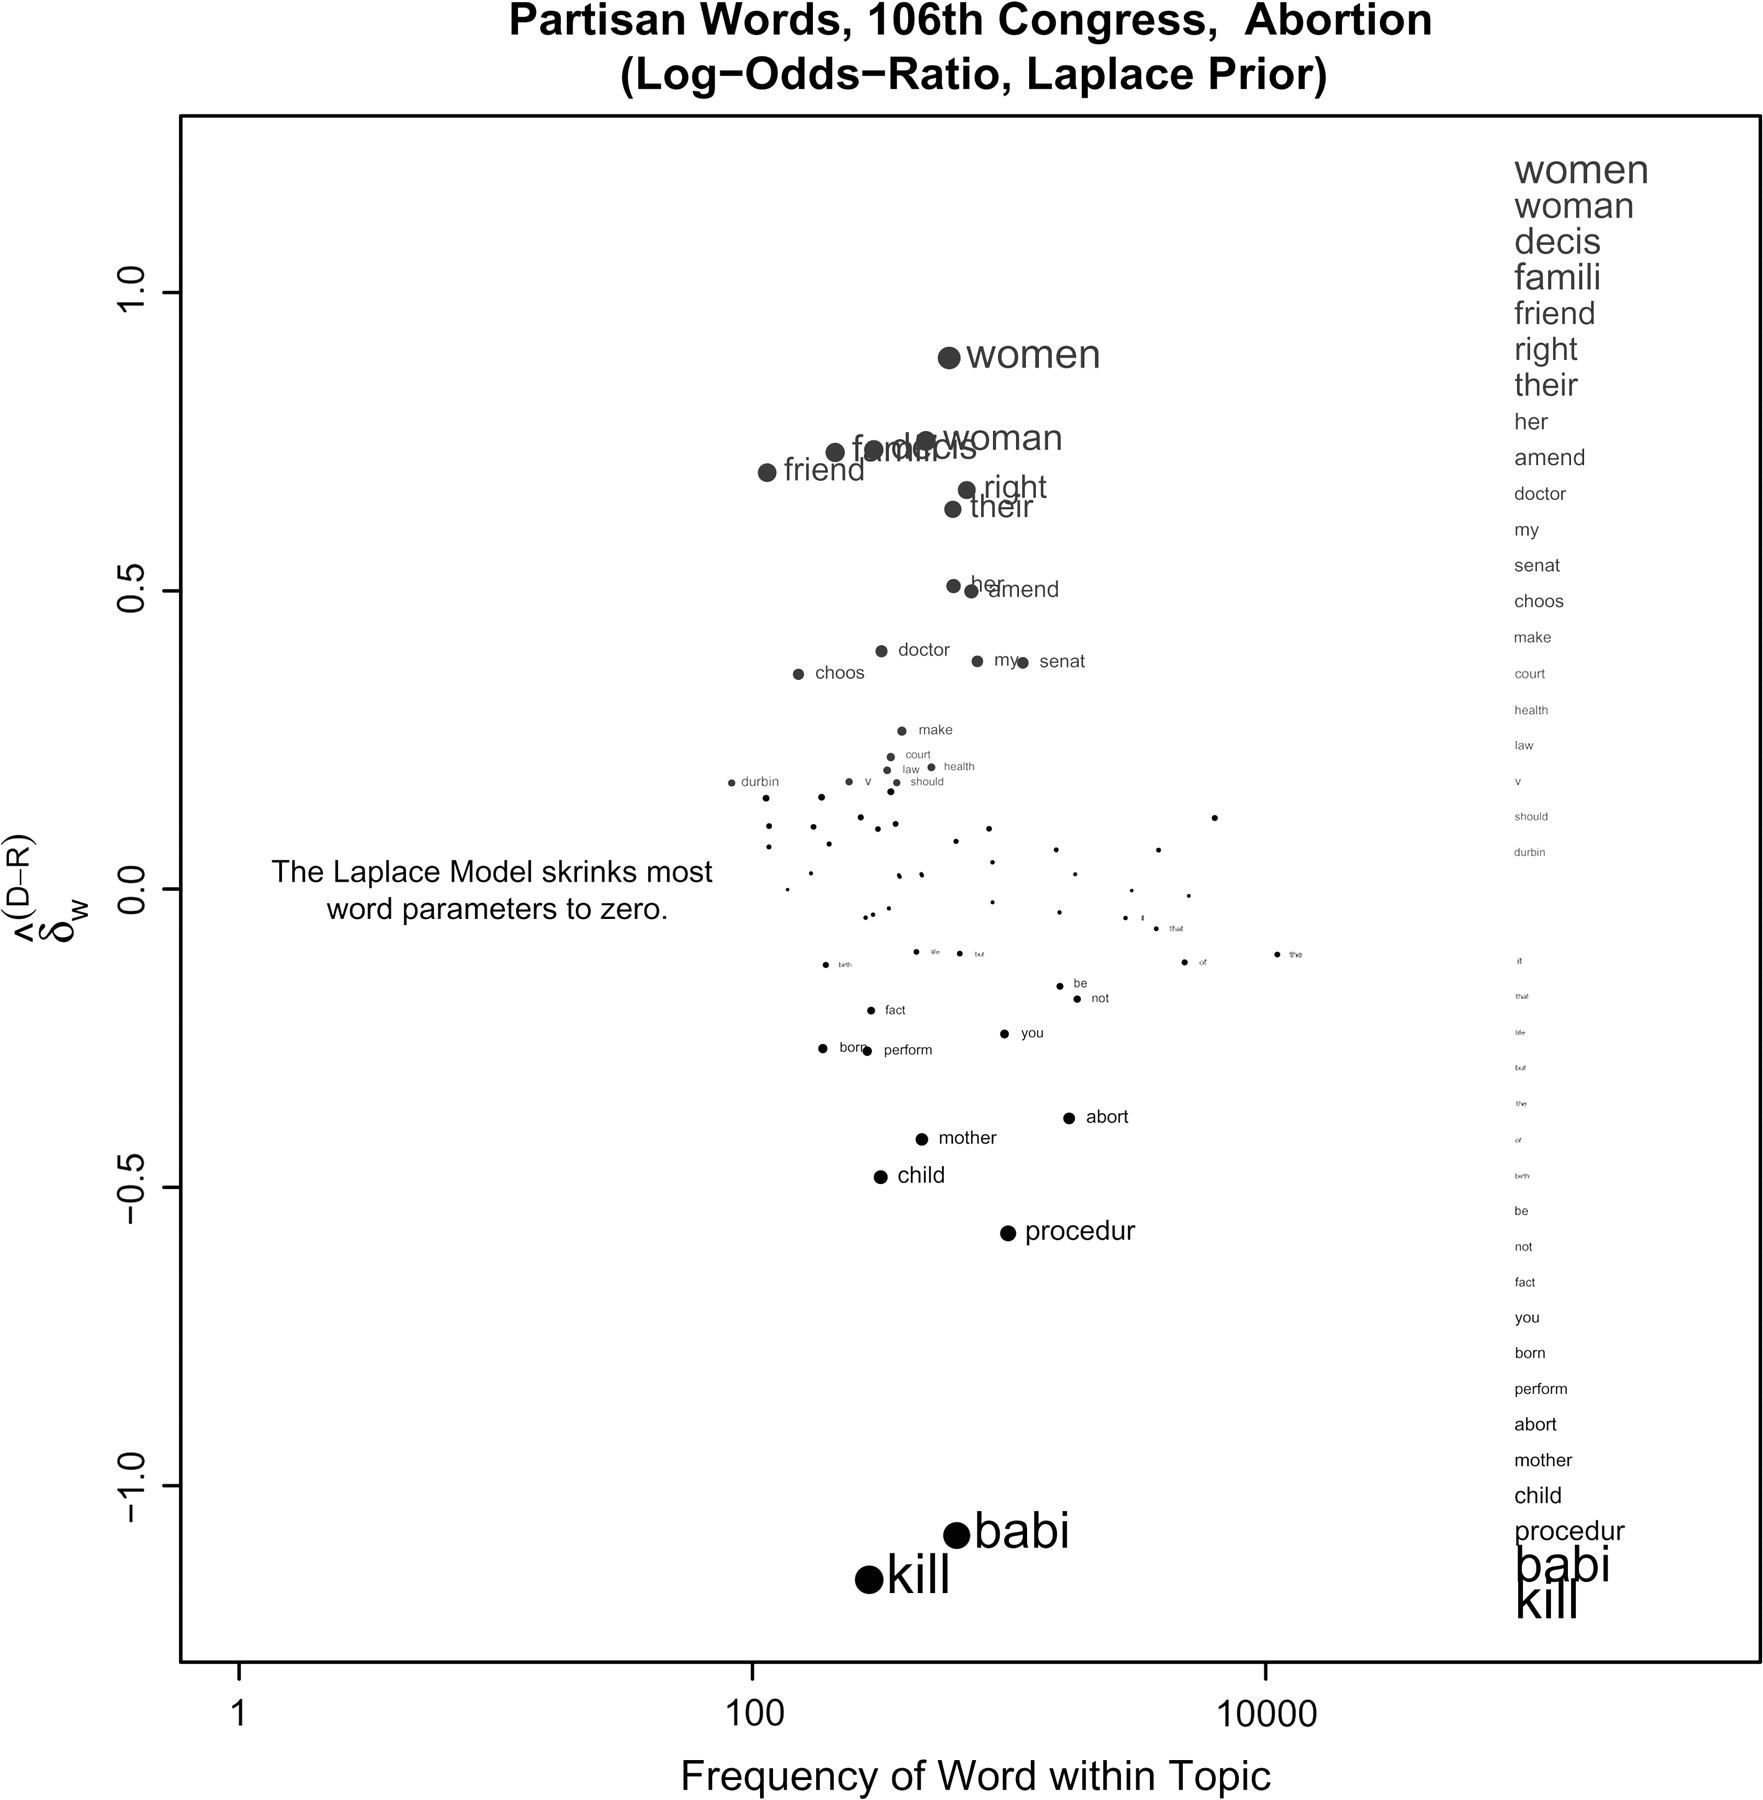
\includegraphics[scale=.2]{pictures/fightin1}}

{\footnotesize An additional prior means that words whose partisanship is not clear will receive partisan contrasts that are exactly zero. Identifying important words is now easier (Monroe et al. 2009).} 

\slide{Lexical Instability}

\centerline{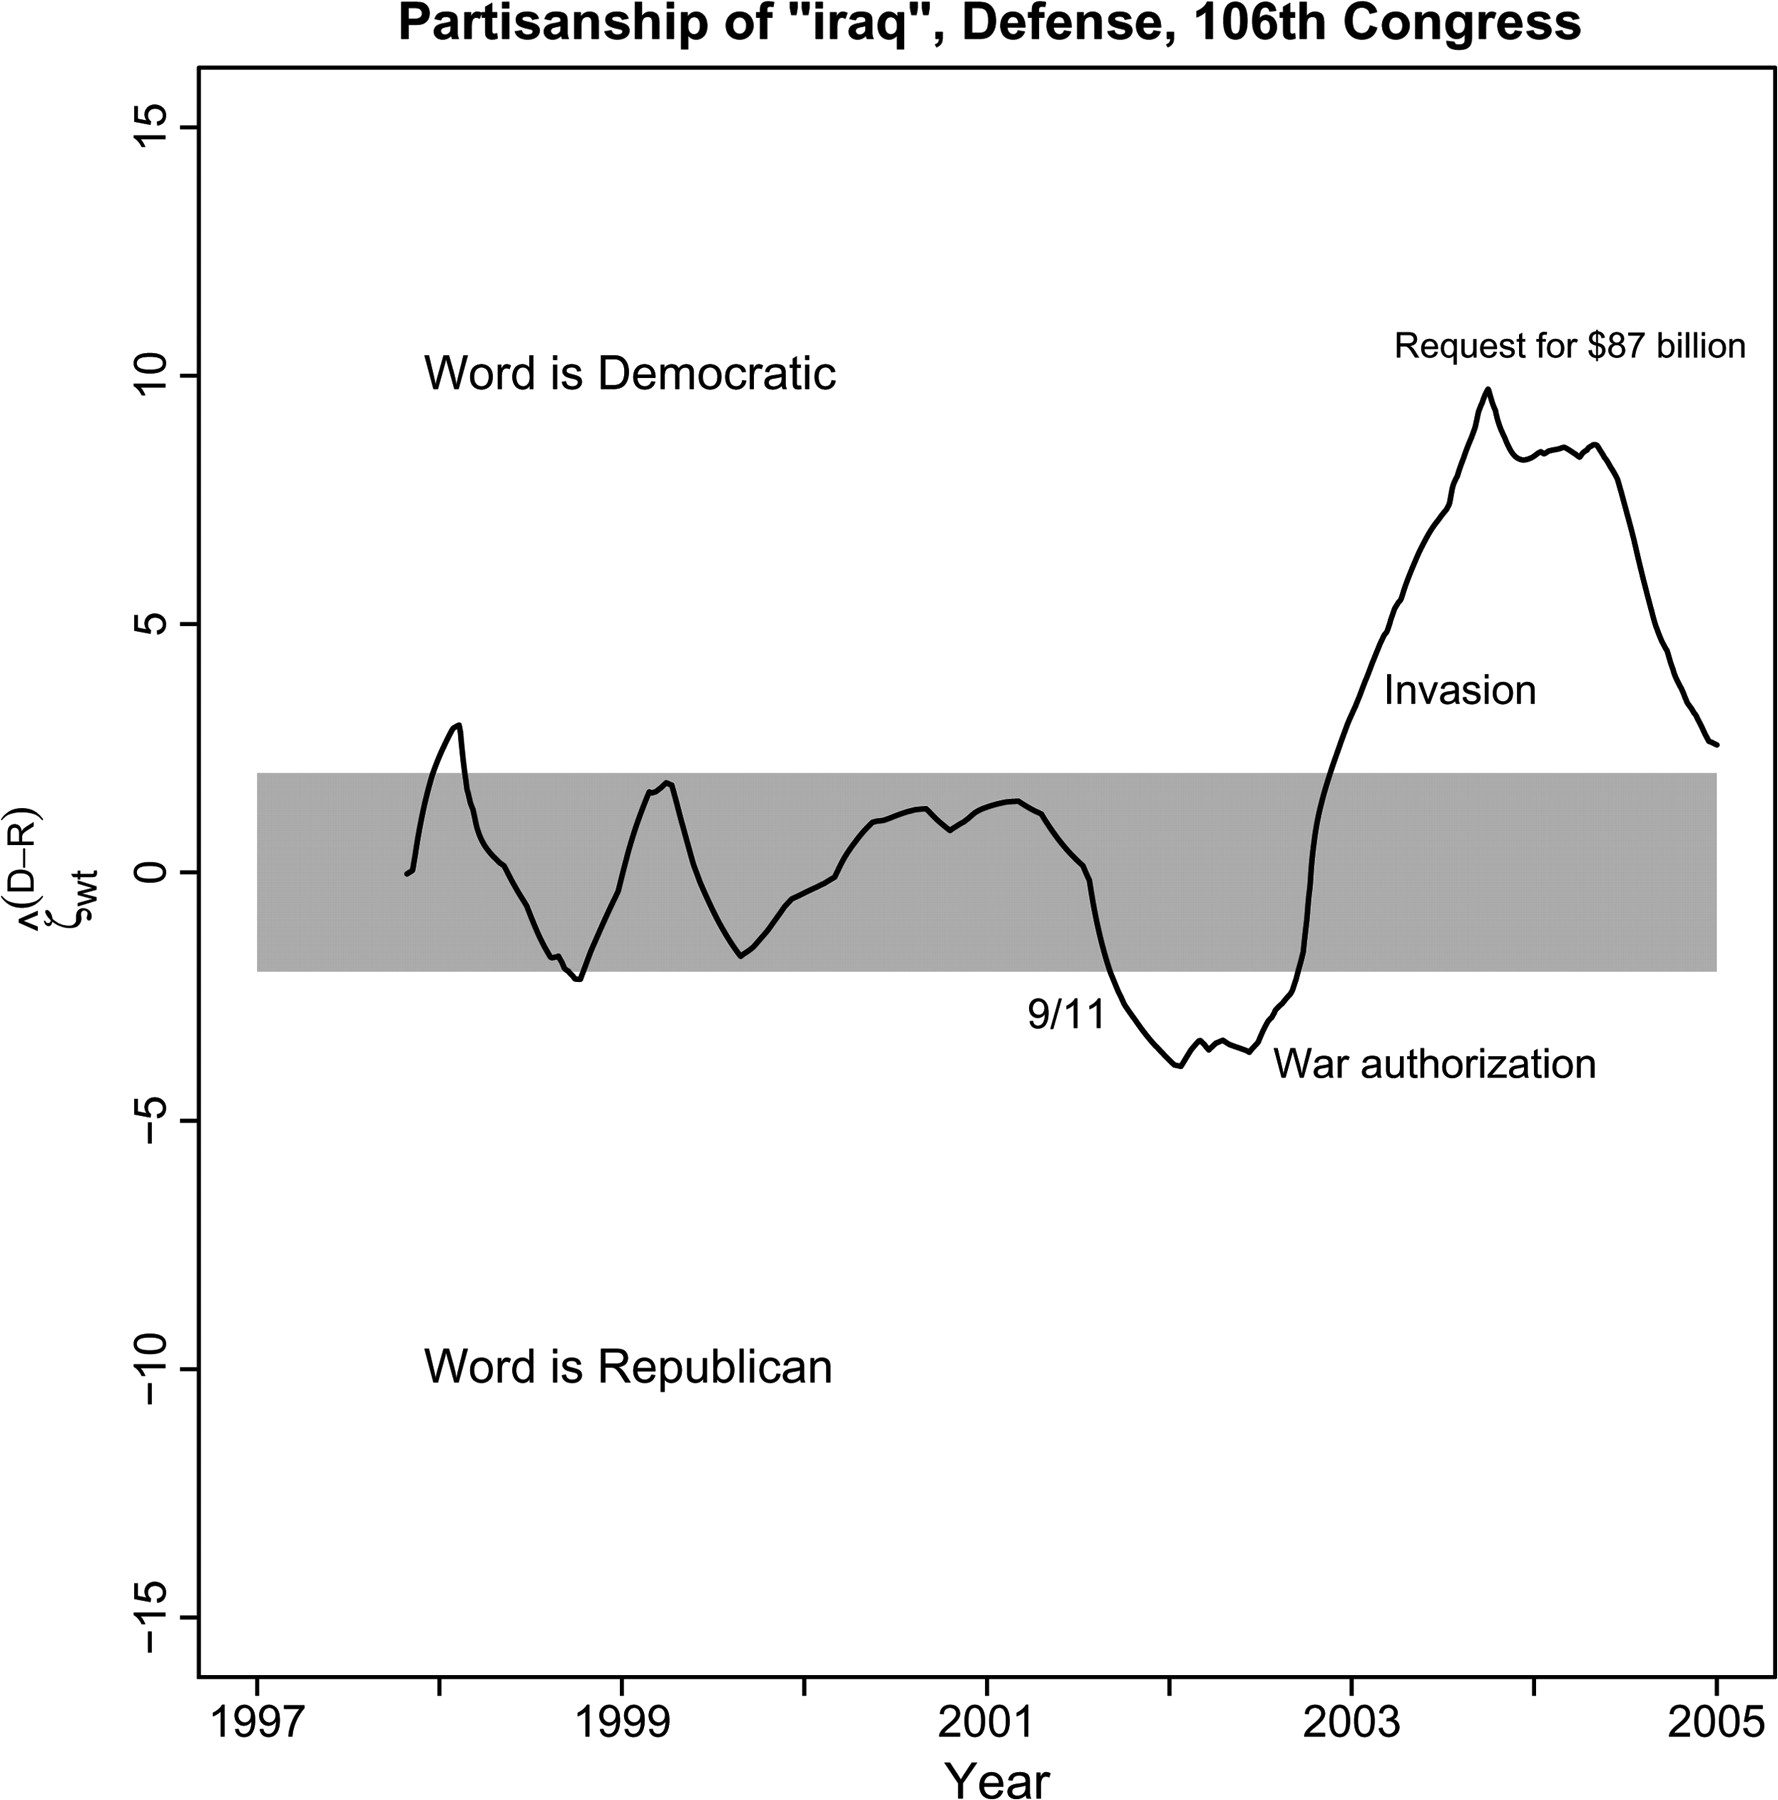
\includegraphics[scale=.21]{pictures/fightin2}}

%%%%%%%%%

\slide{Evaluation case study}

For large numbers of categories, evaluation -- even constructing a reliable confusion matrix -- can be tiresome

For automated classifiers only, a lazy method is possible (King and Lowe, 2003)

\slide{Evaluation case study: events}
                                                                
Russian artillery south of the Chechen
capital Grozny blasted Chechen
positions overnight before falling silent
at dawn, witnesses said on Tuesday.

\noindent                                                                       
Israel said on Tuesday it sent
  humanitarian aid to
Colombia where a massive
  earthquake last week
killed at least 938 people and injured 400.

\slide{Event data extraction}

                                                                                                                               
\mkred{Russian artillery}$^{\,\mathsf{S}}$ south of the Chechen
capital
Grozny \mkgreen{blasted}$^{\,\mathsf{223}}$ \mkblue{Chechen
positions}$^{\,\mathsf{T}}$ overnight before falling silent
at dawn, witnesses said on Tuesday.

\noindent                                                          
\mkred{Israel}$^{\,\mathsf{S}}$ said on Tuesday it \mkgreen{sent
  humanitarian aid}$^{\,\mathsf{073}}$ to
\mkblue{Colombia}$^{\,\mathsf{T}}$ where a \mkred{massive
  earthquake}$^{\,\mathsf{S}}$ last week
\mkgreen{killed}$^{\,\mathsf{222}}$ at least \mkblue{938~
people}$^{\,\mathsf{T}}$ and injured 400.
~\\

\slide{Event data extraction}

                                                                                                                               
\mkred{Russian artillery}$^{\,\mathsf{S}}$ south of the Chechen
capital
Grozny \mkgreen{blasted}$^{\,\mathsf{223}}$ \mkblue{Chechen
positions}$^{\,\mathsf{T}}$ overnight before falling silent
at dawn, witnesses said on Tuesday.

\noindent                                                          
\mkred{Israel}$^{\,\mathsf{S}}$ said on Tuesday it \mkgreen{sent
  humanitarian aid}$^{\,\mathsf{073}}$ to
\mkblue{Colombia}$^{\,\mathsf{T}}$ where a \mkred{massive
  earthquake}$^{\,\mathsf{S}}$ last week
\mkgreen{killed}$^{\,\mathsf{222}}$ at least \mkblue{938~
people}$^{\,\mathsf{T}}$ and injured 400.
~\\
{\large
\begin{center}
\texttt{20010901 RUS CHE 223}\\
\texttt{20020804 ISR COL 073}\\
\texttt{20020804 --- COL 222}
\end{center}
}
\slide{Dyadic event data (Serbia-Bosnia)}

\begin{center} 
{\footnotesize
\begin{tabular}{rrr} \toprule
Week       & Code & Description \\ \midrule
1995-07-11 & 211 & SEIZE POSSESSION \\
 & 212 & ARREST PERSON \\
 & 223 & MILITARY ENGAGEMENT \\ \midrule
1995-07-12 & 211 & SEIZE POSSESSION \\
 & 223 & MILITARY ENGAGEMENT \\
 & 173 & SPECIF THREAT \\
 & 191 & CANCEL EVENT \\
 & 211 & SEIZE POSSESSION \\
 & 095 & PLEAD \\
 & 111 & TURN DOWN \\
 & 212 & ARREST PERSON \\
 & 081 & MAKE AGREEMENT \\
 & 023 & NEUTRAL COMMENT \\
 & 032 & VISIT \\
 & 031 & MEET \\ \bottomrule
\end{tabular}
}
\end{center}

\newpage

\slide{Scaled dyadic event data}

\begin{center} 
{\footnotesize
\begin{tabular}{rrr} \toprule
Week       & Code & Score [-10,10) \\ \midrule
1995-07-11 & 211 & -9.2 \\
 & 212 & -9.0 \\
 & 223 & -10.0 \\ \midrule
1995-07-12 & 211 & -9.2 \\
 & 223 & -10.0 \\
 & 173 & -7.0 \\
 & 191 & -2.2 \\
 & 211 & -9.2 \\
 & 095 & 1.2 \\
 & 111 & -4.0  \\
 & 212 & -9.0 \\
 & 081 & 6.5 \\
 & 023 & -0.2 \\
 & 032 & 1.9 \\
 & 031 & 1.0 \\ \bottomrule
\end{tabular}
}
\end{center}

\slide{The human elements}

\textit{Coders} read newswire and extract events\\ \mkgrey{(e.g. GEDS projects, Swisspeace)}

\textit{Experts} assign scores to event types\\
\mkgrey{(e.g. Goldstein 1995, Shellman 2004)}

\textit{Analysts} aggregate and infer conflict dynamics\\ \mkgrey{(Goldstein \& Pevehouse 1997, Pevehouse \& Goldstein 1999)}

%\slide{(Really) old problems}
%
%Equivalences: 
%\ita
%\itm \textbf{-10} $\approx$ 1 mil. action = 2 demands = 5 accusations
%\itz
%Cancellations: 
%\ita
%\itm ~~\textbf{0}~~ $\approx$ 1 demo + 1 agreement = 1 decline to comment
%\itz
%More reports made bad things worse?
%
%~\\
%(see also Yonamine, 2012 for a discussion)
%%Are these numbers right? (Bond et al. 2003, Shellman 2004)
%
%\slide{Prescription? Just use the counts}
%
%Well ok, but\ldots
%\ita
%\itm Univariate count data analysis can be tricky %\pause
%\itm Time series count data analysis is \textit{always} tricky %\pause
%\itm Multivariate time series count data analysis is
%an \textit{open statistical problem}
%\itz
%
%\slide{Scaling, event data style}
%~\\
%\centerline{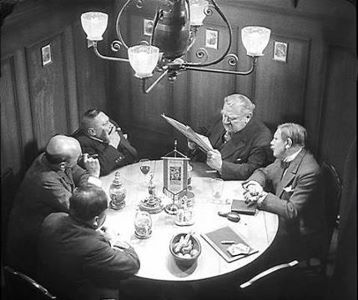
\includegraphics[scale=1]{smoky-room}}
%\vfill
%\centerline{\color{gray}(Goldstein 1995, Bond et al. 2003, Shellman 2004)}
%
%
%
%\slide{Alternative: Distinguish reporting}
%
%\centerline{\includegraphics[scale=.95]{fatn}}
%
%\slide{\ldots from what is reported}
%
%\centerline{\includegraphics[scale=.95]{fatav}}
%

\slide{Evaluating an event data system}

Two aspects of event type evaluation\\ \mkgrey{(King and Lowe 2003)}:
\ita
\itm If machine says it's a use of force, is it really?\\
{(Precision / specificity)}
\itm If it's a use of force, will the machine say it is? \\
{(Recall / sensitivity)} 
\itz

~\\
{\large
\centerline{$P(T \mid M=\text{"223"})$ ~~~vs.~~~ $P(M \mid T=\text{"223"})$}
}

\slide{Evaluating precision}

To estimate $P(T \mid M)$
\ita
\itm 1. Run the machine over all news leads 
\itm 2. Select an equal number of examples from each machine assigned category M
\itm 3. Identify their true event type T
\itz

Boring (code 711 leads from >150 event types sampled from $P(M)$) but straightforward


\slide{Evaluating recall}

We need a gold standard T, but\ldots

\textrm{``of the 45,000 events coded coded by
the VRA Reader from news leads on the former Yugoslavia, it found
10,605 neutral comments but only 4 apologies and 35 threats of
military attack.''}

\vfill
Coders might have to wade through $\sim$2500 comments to find an apology and $\sim$ 300 comments to find a threat of force.

and we're lazy\ldots

\slide{Solution}

Stratified sampling
\ita
\itm Choose events according to what category the machine put them in
\itm -- this is biased!
\itm Correct for the bias
\itz 

\slide{Recall from precision plus computation}
{\large
\begin{align*}
 P(M\mid T)   & = \frac{P(T\mid M)P(M)}{P(T)}
\end{align*}
}
\pause
P(M) is just the event type \textit{tabulation}
\ita
\itm \ldots run the machine on all 45,000 leads
\itz \pause
P(T) is a normalizing constant.


%\slide{Targeted evaluation}
%
%For many applications we don't require few mistakes
%\ita
%\itm \ldots just few mistakes \textit{about conflict and cooperation levels}
%\itz
%
%\pause
%So we evaluate in terms of \textit{expected Goldstein scores}
%{\large
%\begin{equation*}
%  g_i = E[G_{j|i}]=\sum_{j=1}^J G_{j|i}\,P(M=j \mid T=i),
%\end{equation*}
%}

\slide{Undergrads vs. the machine}

{\small
\begin{center}  
\begin{tabular}{r|llll|llll}
            & \multicolumn{4}{c}{All Codes} & \multicolumn{4}{c}{WEIS Codes} \\
& $M$ & $U^{(1)}$ & $U^{(2)}$ & $U^{(3)}$ & $M$ & $U^{(1)}$ & $U^{(2)}$ & $U^{(3)}$ \\
$w=1$    &     &     &     &       &      &     &     & \\
detailed    & .26 & .32 & .23 & .26   &  \textbf{.25} & \textbf{.44} & \textbf{.25} & \textbf{.37} \\
aggregate   & .55 & .55 & .39 & .48   &  \textbf{.62} & \textbf{.62} & \textbf{.48} & \textbf{.62} \\
            &     &     &     &       &      &     &     &  \\
$w=P(t)$    &     &     &     &      &      &     &    & \\
detailed    & .52 & .48 & .35 & .42   &  .55 & .64 & .35 & .68 \\
aggregate   & .65 & .70 & .53 & .64   &  .70 & .72 & .56 & .65 \\
            &     &     &     &       &      &     &     &  \\
$w=1/\sqrt{P(t)}$&&       &     &       &      &     &     & \\
detailed    & .36 & .44 & .33 & .41   &  .37 & .62 & .34 & .67 \\
aggregate   & .59 & .66 & .49 & .62   &  .64 & .68 & .53 & .63 \\
            &     &     &     &       &      &     &     &  \\
\end{tabular}
\end{center}
}


\slide{Summary}

Two points about evaluating machine 
\ita
\itm With a machine classifier we can be lazier than usual when constructing the confusion matrix
\itm Stratification allows you choose an evaluation score that reflects the cost of mistakes in the task
\itm The `inversion' methods discussed yesterday can be applied here too\ldots 
\itz

\slide{Classification: Good Old Logit}

It is tempting to go with methods we know (disciminative style)
\begin{eqnarray*}
\hat{\theta}_{k|w} &=& P(Z=k \mid W_1 \ldots W_V)\\
         &=& \text{logit}^{-1}(\alpha + \beta_1 W_1 + \beta_2 W_2 + \ldots)
\end{eqnarray*}

This is a bad idea
\ita
\itm Why?
\itz

\slide{Bad Old Logit}

The number of word types V is almost much larger than the number of documents D
\ita
\itm Many more `cases' than `variables'
\itm \textit{and} no constraint on possible solutions
\itz

We need \textit{serious} regularisation\ldots

\slide{Wrapping up}



Two approaches
\ita
\itm Discriminative: Model $P(Z \mid \{W\}, \beta) = \theta_{z|w}$ directly
\itm Generative: Model $P(\{W\} \mid Z, \beta)$ and $P(Z)=\theta_z$, then get $P(Z \mid \{W\}, \beta) = \theta_{z|w}$ via Bayes theorem
\itz
For pure blackbox efficiency, go for the first!


\end{document}




%%%%%%%%%%%%%%%%%%%%%%%%%%%%%


































\slide{Ideological Position and SVM}

Support Vector Machines are the state of the art for classification accuracy (just)
\ita
\itm Non-statistical (maximum margin) method
\itm Computationally demanding
\itm Non-intuitive parameterization
\itz

Question: What are the ideological positions of senators?

Yu et al. use the 25 most liberal and 25 most conservative senators (chosen via DNOMINATE scores) to train a SVM classifier to classify senators by their speeches:


%\slide{Ideological Position and SVM}

%\centerline{\includegraphics[scale=.9]{pictures/yu-5}}

\slide{Ideological positions}

Up to 94\% correct classification on these 50 senators 

Only up to 64\% correct classification trained and tested on moderate senators (the middle 50)

\slide{A Theory of Moderates (1)}

\begin{quotation}
``[This is] a new way to think about 
moderate senators which uncovers a hidden assumption in the spatial representation of 
ideologies. According to the Poole-Rosenthal approach, the ideological position of 
members of Congress is identical to their ideal point in a multi-dimensional. 
But once we 
fix an ideal point, moderate ideological positions are just as well-defined and precise as 
``extreme'' positions.'' 
\end{quotation}

\slide{A Theory of Moderates (2)}

\begin{quotation}
``There is, however, a different way to conceptualize moderates. We 
are not aware of a formal representation of this idea, but it does appear from time to time 
in popular political discourse. The idea here is that moderate liberals and conservatives 
do not constitute a separate position, but are simply \textsl{more blurry} versions of their extreme 
counter-parts.''
\end{quotation}

\slide{A Theory of Moderates (3)}

Predictions:
\ita 
\itm If moderates are `blurry' extremists then a classifier trained on moderate example would do less in classifying both moderates and extremists
\itm If moderate is a position, then a classifier trained on moderate example would do very well on moderates and not well on extremists
\itz

\slide{A Theory of Moderates (4)}

\centerline{\includegraphics[scale=.9]{pictures/yu-5}}

\slide{A Theory of Moderates}

\centerline{Do we believe this?}

\slide{}



%:RESIDUAL MATERIAL

%%%%%%%%%%%%%%%%%%%%%%%
%% part 2 %%%%%%%%%%%%%
%%%%%%%%%%%%%%%%%%%%%%%



%%%%%% Measurement here


\slide{Measurement models}

Substantive assumption 
\begin{quotation}
\noindent
Unobserved $\theta$ \textsl{causes} observations $W_1, W_2, W_3,\ldots, W_V$ 
\end{quotation}
 Statistical assumption 
\begin{quotation}
$P(W_1,\ldots, W_V \mid \theta) ~=~ \prod_w^{V} P(W_w \mid {\theta})$ 
\end{quotation}
Once $\theta$ is known, variation in $W_1, W_2, W_3,\ldots, W_V$ 
is random.

\slide{Measurement models}

General Principle:
\ita
\itm Effects of a common cause will be correlated, until it is conditioned on, or controlled for
\itz

You've seen this before, e.g
\ita
\itm good regression models make observations random, conditional on the explanatory variables
\itz


\slide{Measurement Models}

Measurement model: 
\ita
\itm Fit a model of $W_1 \ldots W_V \Leftarrow \theta$\\
then \textit{reverse} it to get an estimate of $\theta$
\itz
Examples:
\ita
\itm Factor Analysis
\itm Latent Class analysis
\itm Item Response Theory
\itm Structural Equation Models
\itz

\slide{Measurement Models}

Advantage: Requires no information about $Z$s or $\theta$s

Disadvantage: Leans heavily on functional and distributional assumptions

Let's look at some possible assumptions\ldots 

\slide{How might $\theta$ affect words?}

word prob. depends on \textit{identity} of $\theta$\\
 (via a category label Z)

word prob. depends on the \textsl{magnitude} of $\theta$

word prob. depends on the \textsl{distance} of $\theta$ from a point



%%%%%%%%%%%%%% scaling %%%%%%%%%%%%%

\slide{Of Left and Right}


Spatial politics assumptions:
\ita
\itm Policy preferences are \textit{positions} or \textit{ideal points} on policy \textit{dimensions}
\itm There exists a \textit{low-dimensional space} that explains the multitude of positioning information available in observations of politics
\itz
Take everyday talk about 'left' and 'right' seriously.

Political representation is effective -- democratic, legitimate -- if politicians' preferences have the \textsl{right relationship} to citizens' preferences.

\slide{Raw Materials of Left and Right}

Quantitative positioning information:
\ita
\itm Votes in a legislature (obvious, but biased)
\itm Answers to survey questions (unbiased but only sometimes possible)
\itm Structured qualitative analysis of manifestos (e.g. Pellican, Krouwel)
\itm Counts of policy promises or assertions in a manifesto or speech (Budget et al.)

\itm Frequencies of individual words
\itz

\slide{Of Left and Right}

\begin{center}
\includegraphics[scale=.3]{pictures/local-maastricht}
\end{center}


Keiskompass (see also Wahl-o-mat).


\slide{Senate Speeches (Monroe et al.)}

\begin{center}
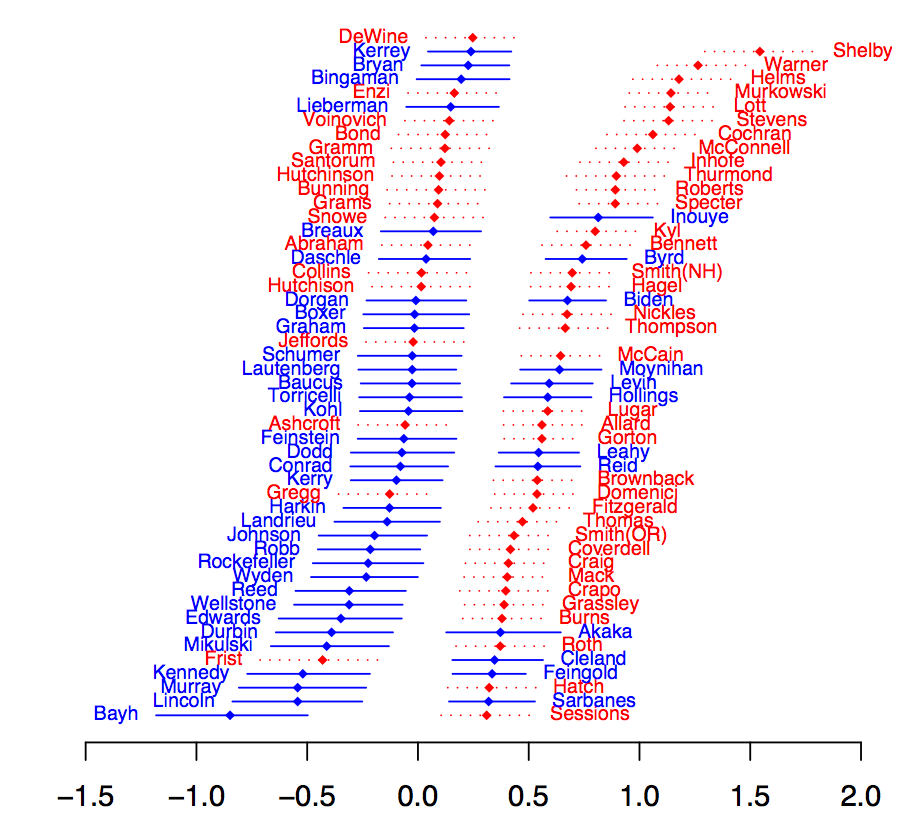
\includegraphics[scale=.2]{pictures/senator-ip-monroe-maeda}
\end{center}

\slide{UK and IE Parties on the Economy}

\begin{center}
\includegraphics[scale=.25]{pictures/wordscores-uk-ie}
\end{center}


\slide{2009 IE Budget Debate}

\begin{center}
\includegraphics[scale=.6]{pictures/clean-snap}
\end{center}

\slide{Scaling Model (Proksch and Slapin)}

Assumptions about $P(W_1\ldots W_V \mid \theta)$
\begin{align*}
\log  \lambda_{ij} &~=~ \psi_j ~+~ \beta_j\theta_i ~+~  \alpha_i
\end{align*}

$\theta_i$ is the expressed position of a text

\slide{Scaling Model (Proksch and Slapin)}

Assumptions about $P(W_1\ldots W_V \mid \theta)$
\begin{align*}
\log  \lambda_{ij}  &~=~ \psi_j ~+~ \beta_j\theta_i ~+~  \alpha_i
\end{align*}
 
$\alpha_i$ is a constant term controlling for document length 

\slide{Scaling Model (Proksch and Slapin)}

Assumptions about $P(W_1\ldots W_V \mid \theta)$
\begin{align*}
\log  \lambda_{ij}  &~=~ \psi_j ~+~ \beta_j\theta_i ~+~  \alpha_i
\end{align*}

 The \textsl{sign} of $\beta_j$ represents the \textsl{ideological direction} of $W_j$

\slide{Scaling Model (Proksch and Slapin)}

Assumptions about $P(W_1\ldots W_V \mid \theta)$
\begin{align*}
\log  \lambda_{ij}  &~=~ \psi_j ~+~ \beta_j\theta_i ~+~  \alpha_i
\end{align*}

 The \textsl{magnitude} of $\beta_j$ represents the \textsl{sensitivity} of the word to ideological differences among speakers or parties

\slide{Scaling Model (Proksch and Slapin)}

Assumptions about $P(W_1\ldots W_V \mid \theta)$
\begin{align*}
\log  \lambda_{ij}  &~=~ \psi_j ~+~ \beta_j\theta_i ~+~  \alpha_i
\end{align*}

$\psi_j$ is a constant term for the word (larger for high frequency words).


\slide{Scaling Model (Proksch and Slapin)}
\begin{center}
\includegraphics[scale=.3]{pictures/log-lambda.pdf}\hfill
\includegraphics[scale=.3]{pictures/lambda.pdf}
\end{center}

The underlying Poisson regression model reflects a \textit{multiplicative} relationship between position and words used

\slide{Marginal Effects}

British National Party manifesto for 2009 EU elections

\slide{Marginal Effects}

\footnotesize
Immigration is out of control.
\normalsize

\slide{Marginal Effects}

\footnotesize
Immigration is out of control.
\textbf{Britain's population is now over 60 million and rising, solely due to immigration.}
\normalsize

\slide{Marginal Effects}

\footnotesize
Immigration is out of control.
Britain's population is now over 60 million and rising, solely due to immigration.
\textbf{Not only is Britain increasingly overcrowded but the fact is that a country is the product of its people  and
if you change the people you will inevitably change the nature of the country.}
\normalsize

\slide{Marginal Effects}

\footnotesize
Immigration is out of control.
Britain's population is now over 60 million and rising, solely due to immigration.
Not only is Britain increasingly overcrowded but the fact is that a country is the product of its people  and
if you change the people you will inevitably change the nature of the country.
\textbf{We want Britain to remain - or return to - the way it has traditionally been.}
\normalsize

\slide{Marginal Effects}

\footnotesize
Immigration is out of control.
Britain's population is now over 60 million and rising, solely due to immigration.
Not only is Britain increasingly overcrowded but the fact is that a country is the product of its people  and
if you change the people you will inevitably change the nature of the country.
We want Britain to remain - or return to - the way it has traditionally been.
\textbf{We accept that Britain will always have ethnic minorities and 
have no problem with this as long as they remain minorities and
neither change nor seek to change the fundamental culture and identity of the indigenous peoples of the British Isles.}
\normalsize

\slide{Marginal Effects}

\footnotesize
\ldots fundamental culture and identity of the indigenous peoples of the British Isles.
\textbf{The current open-door policy and unrestricted uncontrolled immigration is leading to higher crime rates, demand for more housing (driving prices out of the reach of young people), severe strain on the environment, traffic congestion, longer hospital waiting list, lower educational standards, higher income taxes, lower wages, higher unemployment, loss of British identity, a breakdown in community spirit, more restrictive policing, higher council tax rates, a shortage of council homes, higher levels of stress and unhappiness and a more atomized society.}
\normalsize

\slide{Marginal Effects}

~\\
Are we getting the point yet?

%\itm {sentence counts} (Budge 1994; Elff 2008) 

\slide{}

\begin{center}
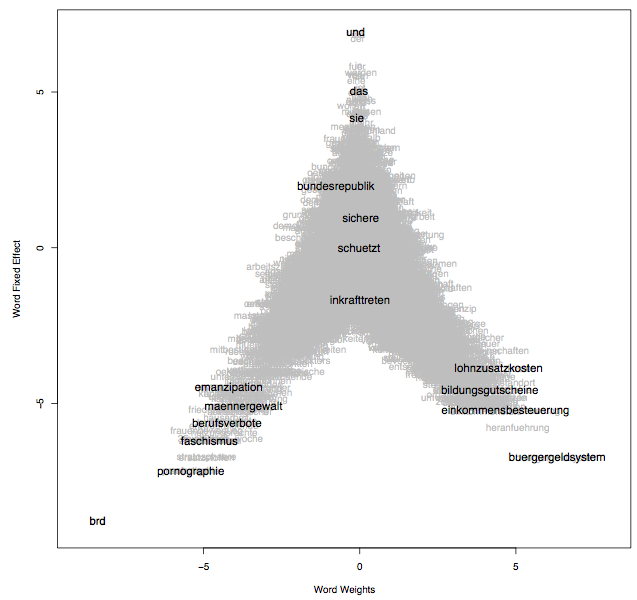
\includegraphics[scale=.35]{pictures/sp-informativeness.png}
\end{center}

\slide{Whew!}

~\\
For the slower version, attend the ECPR Ljubljana Summer School in Methods and Techniques

Questions? Feuer frei!



\slide{Good Old Logit}

It is tempting to go with methods we know (disciminative style)
\begin{eqnarray*}
\hat{\theta}_k &=& P(Z=k \mid W_1 \ldots W_V)\\
         &=& \text{logit}^{-1}(\alpha + \beta_1 W_1 + \beta_2 W_2 + \ldots)
\end{eqnarray*}

This is a bad idea
\ita
\itm Why?
\itz

\slide{Bad Old Logit}

The number of word types V is almost much larger than the number of documents D
\ita
\itm Many more `cases' than `variables'
\itm \textit{and} no constraint on possible solutions
\itz

Options (choose at least one):
\ita
\itm Move to a generative method based on $\theta \longrightarrow$ W
\itm Add constraints on the mapping between W and Z
\itz


\slide{Evaluation: Accuracy, Precision and Recall}

We evaluate using estimates of
\begin{align*}
\text{P}(\hat{Z}=\text{`petitioner'} \mid Z=\text{`petitioner'}) && \text{Recall}  \\
\text{P}(Z=\text{`petitioner'} \mid \hat{Z}=\text{`petitioner'}) && \text{Precision}
\end{align*}
and
\begin{align*}
\text{P}(\hat{Z}=\text{`respondent'} \mid Z=\text{`respondent'}) && \text{Recall}  \\
\text{P}(Z=\text{`respondent'} \mid \hat{Z}=\text{`respondent'}) && \text{Precision}
\end{align*}

where $\hat{Z}$ is assigned by \textit{thresholding} $\theta$

\slide{Event data extraction}
                                                      
Russian artillery south of the Chechen
capital Grozny blasted Chechen
positions overnight before falling silent
at dawn, witnesses said on Tuesday.

\noindent                                                                       
Israel said on Tuesday it sent
  humanitarian aid to
Colombia where a massive
  earthquake last week
killed at least 938 people and injured 400.

\slide{Event data extraction}

                                                                                                                               
\mkred{Russian artillery}$^{\,\mathsf{S}}$ south of the Chechen
capital
Grozny \mkgreen{blasted}$^{\,\mathsf{223}}$ \mkblue{Chechen
positions}$^{\,\mathsf{T}}$ overnight before falling silent
at dawn, witnesses said on Tuesday.

\noindent                                                          
\mkred{Israel}$^{\,\mathsf{S}}$ said on Tuesday it \mkgreen{sent
  humanitarian aid}$^{\,\mathsf{073}}$ to
\mkblue{Colombia}$^{\,\mathsf{T}}$ where a \mkred{massive
  earthquake}$^{\,\mathsf{S}}$ last week
\mkgreen{killed}$^{\,\mathsf{222}}$ at least \mkblue{938~
people}$^{\,\mathsf{T}}$ and injured 400.
~\\

\slide{Event data extraction}

                                                                                                                               
\mkred{Russian artillery}$^{\,\mathsf{S}}$ south of the Chechen
capital
Grozny \mkgreen{blasted}$^{\,\mathsf{223}}$ \mkblue{Chechen
positions}$^{\,\mathsf{T}}$ overnight before falling silent
at dawn, witnesses said on Tuesday.

\noindent                                                          
\mkred{Israel}$^{\,\mathsf{S}}$ said on Tuesday it \mkgreen{sent
  humanitarian aid}$^{\,\mathsf{073}}$ to
\mkblue{Colombia}$^{\,\mathsf{T}}$ where a \mkred{massive
  earthquake}$^{\,\mathsf{S}}$ last week
\mkgreen{killed}$^{\,\mathsf{222}}$ at least \mkblue{938~
people}$^{\,\mathsf{T}}$ and injured 400.
~\\
{\large
\begin{center}
\texttt{20010901 RUS CHE 223}\\
\texttt{20020804 ISR COL 073}\\
\texttt{20020804 --- COL 222}
\end{center}
}
\slide{Dyadic event data (Serbia-Bosnia)}

\begin{center} 
{\footnotesize
\begin{tabular}{rrr} \toprule
Week       & Code & Description \\ \midrule
1995-07-11 & 211 & SEIZE POSSESSION \\
 & 212 & ARREST PERSON \\
 & 223 & MILITARY ENGAGEMENT \\ \midrule
1995-07-12 & 211 & SEIZE POSSESSION \\
 & 223 & MILITARY ENGAGEMENT \\
 & 173 & SPECIF THREAT \\
 & 191 & CANCEL EVENT \\
 & 211 & SEIZE POSSESSION \\
 & 095 & PLEAD \\
 & 111 & TURN DOWN \\
 & 212 & ARREST PERSON \\
 & 081 & MAKE AGREEMENT \\
 & 023 & NEUTRAL COMMENT \\
 & 032 & VISIT \\
 & 031 & MEET \\ \bottomrule
\end{tabular}
}
\end{center}

\newpage

\slide{Scaled dyadic event data}

\begin{center} 
{\footnotesize
\begin{tabular}{rrr} \toprule
Week       & Code & Score [-10,10) \\ \midrule
1995-07-11 & 211 & -9.2 \\
 & 212 & -9.0 \\
 & 223 & -10.0 \\ \midrule
1995-07-12 & 211 & -9.2 \\
 & 223 & -10.0 \\
 & 173 & -7.0 \\
 & 191 & -2.2 \\
 & 211 & -9.2 \\
 & 095 & 1.2 \\
 & 111 & -4.0  \\
 & 212 & -9.0 \\
 & 081 & 6.5 \\
 & 023 & -0.2 \\
 & 032 & 1.9 \\
 & 031 & 1.0 \\ \bottomrule
\end{tabular}
}
\end{center}

\slide{Summed scaled dyadic event data}

\centerline{\includegraphics[scale=.8]{fatsum}}

\slide{The human elements}

\textit{Coders} read newswire and extract events\\ \mkgrey{(e.g. GEDS projects, Swisspeace)}

\textit{Experts} assign scores to event types\\
\mkgrey{(e.g. Goldstein 1995, Shellman 2004)}

\textit{Analysts} aggregate and infer conflict dynamics\\ \mkgrey{(Goldstein \& Pevehouse 1997, Pevehouse \& Goldstein 1999)}

%\slide{(Really) old problems}
%
%Equivalences: 
%\ita
%\itm \textbf{-10} $\approx$ 1 mil. action = 2 demands = 5 accusations
%\itz
%Cancellations: 
%\ita
%\itm ~~\textbf{0}~~ $\approx$ 1 demo + 1 agreement = 1 decline to comment
%\itz
%More reports made bad things worse?
%
%~\\
%(see also Yonamine, 2012 for a discussion)
%%Are these numbers right? (Bond et al. 2003, Shellman 2004)
%
%\slide{Prescription? Just use the counts}
%
%Well ok, but\ldots
%\ita
%\itm Univariate count data analysis can be tricky %\pause
%\itm Time series count data analysis is \textit{always} tricky %\pause
%\itm Multivariate time series count data analysis is
%an \textit{open statistical problem}
%\itz
%
%\slide{Scaling, event data style}
%~\\
%\centerline{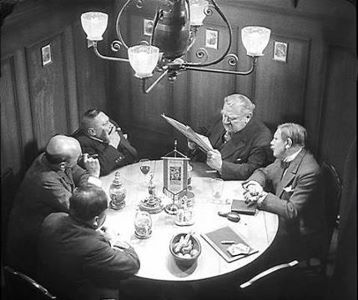
\includegraphics[scale=1]{smoky-room}}
%\vfill
%\centerline{\color{gray}(Goldstein 1995, Bond et al. 2003, Shellman 2004)}
%
%
%
%\slide{Alternative: Distinguish reporting}
%
%\centerline{\includegraphics[scale=.95]{fatn}}
%
%\slide{\ldots from what is reported}
%
%\centerline{\includegraphics[scale=.95]{fatav}}
%

\slide{Evaluating an event data system}

Two aspects of event type evaluation\\ \mkgrey{(King and Lowe 2003)}:
\ita
\itm If machine says it's a use of force, is it really?\\
{(Precision / specificity)}
\itm If it's a use of force, will the machine say it is? \\
{(Recall / sensitivity)} 
\itz

~\\
{\large
\centerline{$P(T \mid M=\text{"223"})$ ~~~vs.~~~ $P(M \mid T=\text{"223"})$}
}

\slide{Evaluating precision}

To estimate $P(T \mid M)$
\ita
\itm 1. Run the machine over all news leads 
\itm 2. Select an equal number of examples from each machine assigned category M
\itm 3. Identify their true event type T
\itz

Boring (code 711 leads from >150 event types sampled from $P(M)$) but straightforward


\slide{A problem evaluating recall}

We need a gold standard T, but\ldots

\textrm{``of the 45,000 events coded coded by
the VRA Reader from news leads on the former Yugoslavia, it found
10,605 neutral comments but only 4 apologies and 35 threats of
military attack.''}

\vfill
Coders might have to wade through $\sim$2500 comments to find an apology and $\sim$ 300 comments to find a threat of force.

and we're lazy (on their behalf)

\slide{A solution}
{\large
\begin{align*}
 P(M\mid T)   & = \frac{P(T\mid M)P(M)}{P(T)}
\end{align*}
}
\pause
P(M) is just the event type \textit{tabulation}
\ita
\itm \ldots run the machine on all 45,000 leads
\itz \pause
P(T) is a normalizing constant.



\slide{Undergrads vs. the machine}

{\small
\begin{center}  
\begin{tabular}{r|llll|llll}
            & \multicolumn{4}{c}{All Codes} & \multicolumn{4}{c}{WEIS Codes} \\
& $M$ & $U^{(1)}$ & $U^{(2)}$ & $U^{(3)}$ & $M$ & $U^{(1)}$ & $U^{(2)}$ & $U^{(3)}$ \\
$w=1$    &     &     &     &       &      &     &     & \\
detailed    & .26 & .32 & .23 & .26   &  \textbf{.25} & \textbf{.44} & \textbf{.25} & \textbf{.37} \\
aggregate   & .55 & .55 & .39 & .48   &  \textbf{.62} & \textbf{.62} & \textbf{.48} & \textbf{.62} \\
            &     &     &     &       &      &     &     &  \\
$w=P(t)$    &     &     &     &      &      &     &    & \\
detailed    & .52 & .48 & .35 & .42   &  .55 & .64 & .35 & .68 \\
aggregate   & .65 & .70 & .53 & .64   &  .70 & .72 & .56 & .65 \\
            &     &     &     &       &      &     &     &  \\
$w=1/\sqrt{P(t)}$&&       &     &       &      &     &     & \\
detailed    & .36 & .44 & .33 & .41   &  .37 & .62 & .34 & .67 \\
aggregate   & .59 & .66 & .49 & .62   &  .64 & .68 & .53 & .63 \\
            &     &     &     &       &      &     &     &  \\
\end{tabular}
\end{center}
}

\newpage 

\slide{Targeted evaluation}

For many applications we don't require few mistakes
\ita
\itm \ldots just few mistakes \textit{about conflict and cooperation levels}
\itz

\pause
So we evaluate in terms of \textit{expected Goldstein scores}
{\large
\begin{equation*}
  g_i = E[G_{j|i}]=\sum_{j=1}^J G_{j|i}\,P(M=j \mid T=i),
\end{equation*}
}

\slide{Targeted evaluation}

\centerline{\includegraphics[scale=.97]{g2cropped}}

\slide{Conclusions for event extraction}

Automated methods are competitive with human coders
\ita
\itm time for some pink slips
\itz 



\end{document}